\subsection{Messungen}

\subsubsection{Modell}

%\begin{figure}[h!]
%	\centering
%	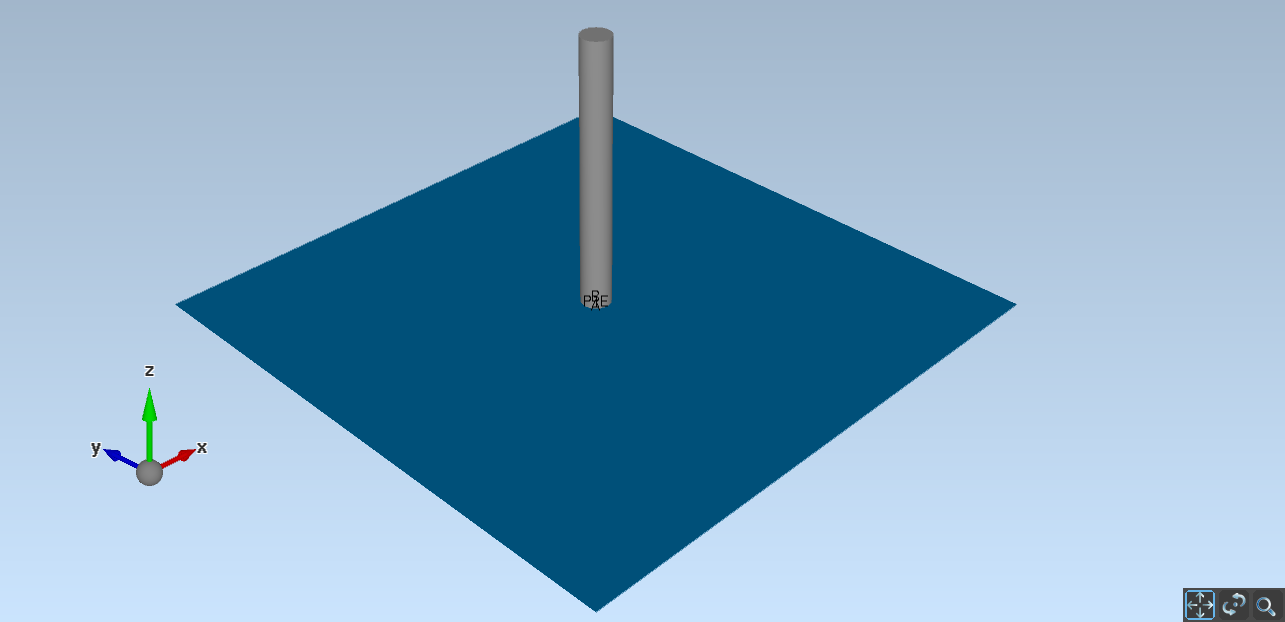
\includegraphics[width=0.5\textwidth]{../fig/plt/monopol_a_sim_3d_model.png}
%	\caption{}
%\end{figure}

\clearpage
\subsubsection{Messergebnisse}

\begin{figure}[h!]
	\begin{subfigure}[t]{0.45\textwidth}
		\centering
		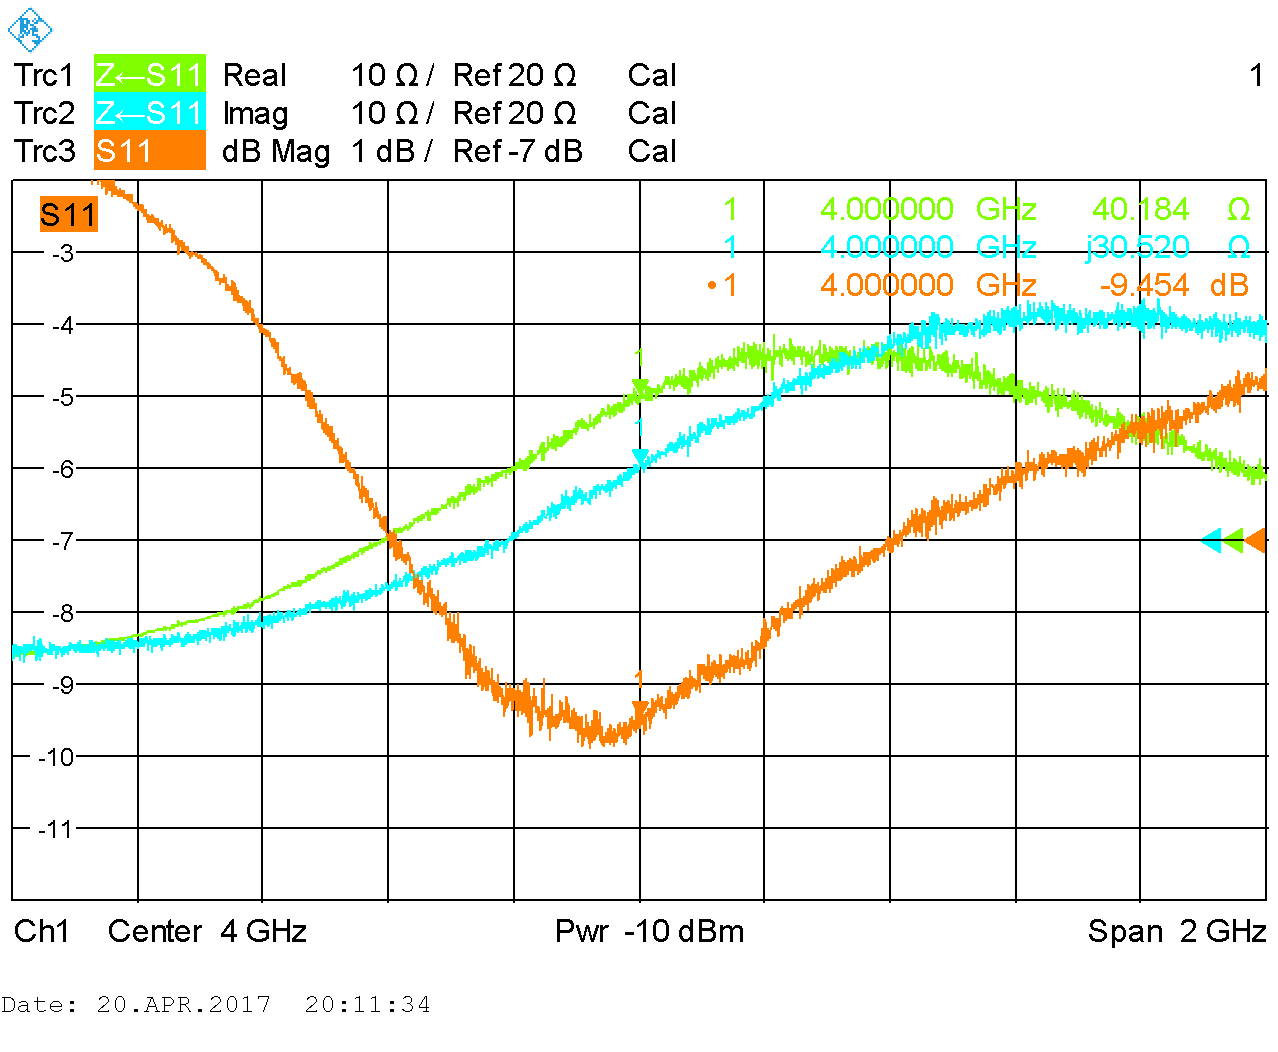
\includegraphics[width=1\textwidth]{../data/measurement/T2.png}
	\end{subfigure}
	\begin{subfigure}[t]{0.45\textwidth}
		\centering
		\begin{tikzpicture}
			\begin{axis}[
				title=\textbf{Reflexion $S_{11}$ (VNA2)},
				width=\linewidth,
				grid=major,
				grid style={dashed,gray!30},
				xlabel={Frequenz [\si{\giga\hertz}]},
				ylabel={$S_{11}$ [\si{\decibel}]},
				x label style={at={(axis description cs:0.5,-0.075)},anchor=north},
				legend style={at={(0.98,0.98)},anchor=north east},
				x tick label style={rotate=90,anchor=east},
				legend columns=1,
				]
				\addplot+[mark=none] table[x=f, y=s11, col sep=comma]{../data/measurement/vna_2_data.txt};
				%\addlegendentry{S11};
			\end{axis}
		\end{tikzpicture}
	\end{subfigure}
	\caption{Messung mit Vector-Nectorwork Analyser.}
\end{figure}

\subsubsection{Messaufbau}

\subsubsection{Messmittel}


